\chapter{Rastreamento de olhar}

Rastreamento de olhar consiste em técnicas para determinar a direção do olhar, ou seja, determinar onde determinada pessoa está olhando, a partir da posição da íris.

Algumas partes do olho humano, que estão representadas na figura $\ref{fig:olho}$,  são as seguintes$\cite{lidade}$:

\afterpage{
%assim o footnote funciona http://blog.peschla.net/2012/11/latex-footnotes-in-captions/
\begin{figure}
\begin{center}
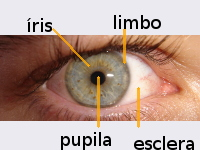
\includegraphics[scale=1]{imagens/eye.jpg}
\caption[]{Regiões do olho. Adaptado de \protect \footnotemark}
\label{fig:olho}
\end{center}
\end{figure}
\footnotetext{\url{http://commons.wikimedia.org/wiki/File:My_eye.jpg}}
}

\begin{itemize}

\item \textbf{pupila}: a abertura que permite a entrada de luz no o olho.
\item \textbf{íris}: o músculo colorido que controla o diâmetro da pupila.
\item \textbf{esclera}: tecido branco protetor que envolve os restante do olho.
\item \textbf{limbo}: o contorno entre a íris e a esclera.
\end{itemize}

%Ao longo do tempo, diferentes abordagens foram usadas para estimar a posição do olhar. \cite{lupung}. Em 1901 Dodge e Cline desenvolveram o primeiro dispositivo não invasivo de estimação de olhar \cite{lupung}, eles usaram fotografias para registrar movimentos do olho. Até o início da década de 70, o rastreamento de olhar era feito com o uso de lentes de contato ou com fotografias \cite{wnek2008eye}.

%No início da década de 70, passaram-se a gravar o olho com câmeras e identificar eletronicamente regiões no olho. 

Existem algumas abordagens de rastreamento, uma delas é a partir do processamento de imagens em vídeo, também conhecida como rastreamento de olhar baseado em vídeo $\cite{lupung}$. Neste tipo de rastreamento, tentamos localizar o olho na imagem e procuramos a posição relativa da pupila no olho.

Dois tipos de imagem podem ser usados no rastramento baseado em vídeo: imagens no espectro visual ou imagens em infravermelho.

No rastreamento pelo espectro visual, a luz refletida pelos olhos é registrada. Neste caso, a eficiência do rastreamento depende das condições de iluminação do ambiente, o que torna o processo complicado $\cite{lidade}$.

No caso de imagens em infravermelho, não temos esse problema, pois o olho é constantemente iluminado por uma fonte de luz infravermelha, que não é percebida pelo usuário. Uma vantagem desta abordagem é que a pupila reflete boa parte da luz infravermelha recebida, sendo a região mais brilhante do olho na imagem $\cite{lidade}$. Devido ao tamanho, a pupila tem menor chance de ser parcialmente ocultada pelos  cílios do que a esclera, outra região que reflete o infravermelho. %pupila será sempre a região mais brilhante na imagem $\cite{lupung}$: se a fonte de luz estiver alinhada com o olho, a pupila aparecerá branca, caso contrário, estará preta na imagem.

A principal desvantagem é que não é possível usar esse tipo de rastreador ao ar livre durante o dia devido à luz infravermelha do ambiente $\cite{lidade}$.

As técnicas de rastreamento de olhar também variam de acordo com a localização da câmera, que pode ser instalada junto à cabeça do usuário (head-mounted) ou remotamente. No caso do rastreamento head-mounted, o usuário deve usar um acessário equipado com uma câmera que registra as imagens do olho. A figura $\ref{fig:pupil}$ mostra um rastreador desse tipo

\afterpage{
%assim o footnote funciona http://blog.peschla.net/2012/11/latex-footnotes-in-captions/
\begin{figure}
\begin{center}
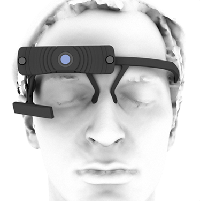
\includegraphics[scale=.7]{imagens/pupil.png}
\caption[]{Um rastreador de olhar acoplado à cabeça. Reproduzido de \protect \footnotemark}
\label{fig:pupil}
\end{center}
\end{figure}
\footnotetext{\url{https://pupil-labs.com/blog/2014-01/new-pupil-pro-headset-capture-software-0-3-7/}}
}

Uma vantagem do rastreamento head-mounted é que a câmera move-se com a cabeça, então mudanças de pose não causam mudanças da posição da pupila na imagem. A desvantagem é a necessidade de usar um equipamento acoplado à cabeça.

\section{Métricas em rastreamento de olhar}

Em algumas aplicações de rastreamento de olhar não estamos interessados apenas na direção do olhar em determinado instante, mas também poderemos querer observar outras características (métricas) relacionadas ao movimento do olhos. As métricas mais específicas são \cite{lupung}:

\begin{itemize}
\item {\bf Fixação e sacada:} Em 1989, Emile Java (oftalmologista francês) observou que os movimentos do olho não ocorrem de forma contínua, e sim de movimentos rápidos, chamados de sacadas, seguidos por breves pausas, conhecidas como fixações;

\item {\bf Área de interesse:} Região no ambiente que está presente no campo visual e que é de interesse em determinada pesquisa;

\item {\bf Duração do olhar:} Duração de um intervalo de tempo em que uma série de fixações está dentro de uma área de interesse;

\item {\bf Caminho de varredura:} localização espacial de uma sequência de fixações.
\end{itemize}